% \documentclass[fleqn,10pt]{wlscirep}
\documentclass[prx,twocolumn,floatfix,superscriptaddress,longbibliography]{revtex4-1}
\usepackage[utf8]{inputenc}
\usepackage[T1]{fontenc}
\usepackage{bm}
\usepackage{tikz}
\usepackage{subfiles}
\usepackage{mathtools}
\usetikzlibrary{shapes,arrows,positioning}
\usepackage{standalone}
\usepackage{amssymb,amsmath,amstext}
\usepackage{amsthm}
\usepackage{bbm}
\usepackage{graphicx}
\usepackage{epstopdf}
\usepackage{color}
\usepackage{appendix}
\usepackage[T1]{fontenc}
\usepackage{bbold}
\usepackage{bbm}
\usepackage{float}
\usepackage{latexsym}
\usepackage{xr-hyper}
\usepackage[colorlinks=true,citecolor=blue,linkcolor=magenta]{hyperref}
\usetikzlibrary{quantikz2}
\usepackage{braket}
\usepackage{physics}
\usepackage{algpseudocode}
\usepackage{placeins}
\usepackage{multirow}
\usepackage{booktabs}
\graphicspath{{./Figures/}}
%\usepackage[latin1]{inputenc}
%\usepackage{hyphenat}

\usepackage{hhline}
%\bibliographystyle{apsrev4-2}
\def\bibsection{\section{\refname}} 
\usetikzlibrary{shapes,arrows}
\renewcommand{\vec}[1]{\boldsymbol{#1}}  % Bold vectors instead of arrow vectors
%\newcommand{\<}{\langle}
%\renewcommand{\>}{\rangle}

\long\def\ca#1\cb{} %Use for commenting out: \ca...\cb

\def\cites#1{XXX Need citation #1 XX}

\begin{document}

\title{Quantum Algorithms for Portflolio Optimisation and Option pricing}

\author{G. Balarezo}
\thanks{e-mail: juan.balarezo@yachaytech.edu.ec}
\affiliation{School of Physical Sciences and Nanotechnology,\\ Yachay Tech University,\\Urcuqui, Ecuador}


\begin{abstract}
Quantum computing has the promise to address computational problems that are considered intractable with our classical computational models. Nevertheless, due to the current limitations of the available quantum hardware, we are still years away from achieving a universal fault-tolerant quantum computer. In the interim, the development of quantum algorithms for specific problems and their implementation on near-term quantum devices is a promising approach. In this work, we review the most promising quantum algorithms for financial applications, focusing on Portfolio Optimisation and Option Pricing. We describe the ideas behind important quantum algorithms such as Variational Quantum Algorithms (VQAs) and Quantum Amplitude Estimation (QAE) and their theoretical performance. We provide an overview of the hardware available for their implementation and discuss the results 
obtained by some study cases, comparing them with their classical counterparts. Finally, we discuss the future prospects of these algorithms in the financial industry.
  \\
  \textbf{Keywords:} Quantum algorithms, Quantum approximate optimization algorithm, Quantum amplitude estimation, Portfolio optimisation, Quantum computing.
\end{abstract}

\maketitle

\section{Introduction}

Quantum computing has become a rapidly growing field of research in recent years, sparking interest from both academic and industrial sectors, including the financial industry in particular \cite{Hassija2020}. The potential of quantum computers to address computational problems that are considered intractable with our classical models of computation \cite{nielsen2010quantum} has driven a considerable amount of research and innovation in the development of Noisy Intermediate-Scale Quantum computers (NISQ) and quantum algorithms capable of leveraging this computational power \cite{Huang2023}. 

These near-term devices, with limited qubit capabilities and high error rates, have shown promising results. Implemented along with classical computers and adequate quantum algorithms, they can offer significant speedups for some important but classically inefficiently solvable problems in areas such as Optimisation \cite{Symons2023}, Stochastic Modelling \cite{Herbert2022}, and Machine Learning \cite{Zeguendry2023}. These advancements are particularly relevant to the financial sector \cite{Egger2020a}, where they could yield substantial speedups in tasks such as portfolio optimisation and option pricing \cite{Hassija2020}. These tasks have a high 
computational cost that coupled with growing complexity of the financial markets, the need for real-time analysis of large amounts of data and fast decision-making \cite{book:2139036}, makes quantum computing 
an attractive option for financial institutions. 

In the Modern Portfolio Theory (MPT) proposed by Markowistz \cite{Markowitz1952}, the goal of portfolio optimisation is to find the best combination of assets that maximises the return for a given level of risk and some constraints. This is a highly constrained quadratic optimisation problem, known to be NP-Hard, which can be formulated in several ways depending on the conditions of the 
investor \cite{Herman2022}. Monte Carlo based models (MC) such as the one proposed by Shadabfar and Cheng \cite{Shadabfar2020} are widely used for minimising risk contributors and maximising asset diversification.

In particular, quantum approaches to portfolio optimisation are gaining significant attention \cite{Quarterly2020}. In 2019 Kerenidis, Prakash and Szilágyi \cite{Kerenidis2019},  proposed a quantum algorithm for the constrained portfolio optimisation problem. Based on an interior point method, this algorithm reduces the optimisation problem to a second order cone program (SOCP). The authors suggest that their algorithm could achieve a $\mathcal{O} (n)$ speedup over  its classical counterpart.

Other approaches such as the variational quantum algorithms (VQAs) \cite{Yuan2019, Cerezo2021, McClean2016, Amaro2022} work by reformulating the portfolio optimisation problem as a 
quadratic unconstrained binary optimisation (QUBO) problem. Glover et al. \cite{Glover2019} covers some methods to reformulate any optimisation problem as a QUBO problem, and Date et al. \cite{Date2019} proposed an algorithm that allows the efficient embedding of a QUBO problem in a quantum annealer.  Using these concepts, Variational Quantum 
Eigensolver (VQE) \cite{Huang2023, McClean2016, Peruzzo2014, Barkoutsos2020, Buonaiuto2023} and Quantum Approximate Optimisation Algorithm (QAOA) \cite{Farhi2014, Blekos2024} have been proposed for portfolio optimisation \cite{Egger2020}. Quantum annealers such as those developed by D-Wave Systems \cite{King2023} are been used for practical implementations of the aforementioned algorithms
\cite{Yarkoni2022, Phillipson2020, Venturelli2019}. Nevertheless, it remains unclear whether these quantum algorithms provide any effective speedup over classical methods for these tasks.

Option pricing is another important task in finance where quantum algorithms have been applied. The implementation of the
Quantum Amplitude Estimation (QAE) algorithm \cite{Woerner2019, Nakaji2020, Stamatopoulos2020, Rebentrost2018} has been proposed for the calculation of the expected value of the option price. This algorithm is

\begin{table*}[t!] 
  \begin{center}
    \caption{\label{Tab:paper_overview} Criteria for the selection of the papers reviewed in this work.}
    \begin{tabular}{c|c|c|c} \hline \hline
\textbf{Metodology} &
  \textbf{Application} &
  \textbf{Algorithm} &
  \textbf{Hardware} \\ \hline
Optimisation &
  \begin{tabular}[c]{@{}c@{}}Portfolio \\ optimisation\end{tabular} &
    \begin{tabular}[c]{@{}c@{}}Approximate \\ Optimisation\\ (SOCP, VQE, QAOA) \\
    \cite{Mazumdar2020}, \cite{Buonaiuto2023}, \cite{Phillipson2020}, \cite{Venturelli2019}  \end{tabular} &
  \begin{tabular}[c]{@{}c@{}}Gate-based quantum computer \\ Quantum Annealer\end{tabular} \\ \hline  
    %\multicolumn{1}{}{  Gate-based quantum computer \\ Quantum Annealer} \\ \hline
Monte Carlo &
  \multicolumn{1}{l|}{\begin{tabular}[c]{@{}l@{}}Option pricing \end{tabular}} &
  \begin{tabular}[c]{@{}c@{}}Search and Count\\ (QAE, QPA, QPE) \\ 
  \cite{Woerner2019},\cite{Nakaji2020}, \cite{Stamatopoulos2020}, \cite{Rebentrost2018}, \cite{Rebentrost2022} \end{tabular} &
\begin{tabular}[c]{@{}c@{}} Gate-based quantum \\ computer\end{tabular} \\ \hline \hline
\end{tabular}
\end{center}
\end{table*}

expected to provide a quadratic speedup over the classical Monte Carlo methods used for this task. 

The aim of this work is to provide a review of the quantum algorithms for specific financial applications, focusing on Portfolio Optimisation and Option Pricing. Table \ref{Tab:paper_overview} provides an overview of the topics covered in this work, as well as the relevant literature reviewed. 

In Sec. \ref{sec:background} we introduce necessary concepts in finance and quantum algorithms. Then, in Sec. \ref{sec:literature1} and Sec. \ref{sec:literature2}  we present a review of relevant literature on quantum algorithms proposed for the aforementioned financial applications. We also 
  introduce the classical methods used for these tasks and compare them with their quantum counterparts.

In Sec. \ref{sec:hardware} we provide an overview of the hardware implementations of these algorithms. Finally, Sec. \ref{sec:discussion} concludes this work and discusses the future prospects of quantum algorithms in the financial industry. 

It is worth mentioning that important surveys have been published on the topic of quantum computing in finance in recent years. Among these, we highlight the works of Orús et al. \cite{Orus2019}, Egger et al. \cite{Egger2020a}, Albareti et al. \cite{Albareti2022}, Herman et al. \cite{Herman2022}, and Herman et al. \cite{Herman2023}, which have been instrumental in the development of this work. We refer the interested readers to these works for a more comprehensive overview of the field.

\section{background}\label{sec:background}
\subsection{Some basics concepts}
\subsubsection{Assets and Portfolio Optimisation}

In finance, an asset is a financial instrument that can be owned by an individual, a corporation, or a country with the expectation that it will provide a future benefit \cite{2023}. Financial assets can include stocks, bonds, commodities, derivatives, etc. 

On the other hand, a portfolio is a set of individual investments that may include a wide range of asset classes. A portfolio is characterised by components such as diversification, risk and return, and asset allocation. The main goal of a portfolio is to diversify investments to achieve some specific objective such as maximising returns, minimising risk, or a balance between them \cite{Wilmott2007}. 
In order to achieve this, portfolio optimisation is used to find the best allocation of assets that fulfils the investor's objectives.

In the original work by Markowitz \cite{Markowitz1952}, a mean-variance portfolio optimisation (MVPO) is proposed, which is widely used used in the financial industry to this day, and whose formulation is presented in this section.

The input for the MVPO is the historical prices and returns of the considered financial assets. An asset range $(1 \leq i \leq N)$ is considered, and a time range $(0 \leq t \leq T)$. 

Then, the first step is to obtain a list $P$ of current prices $P_i$  of the assets of interest.
\begin{equation}
  \label{eq:1}
  P_i = p_i(T)
\end{equation}

In addition, the historical returns of the assets between time $t-1$ and $t$ are calculated as:
\begin{equation}
  \label{eq:2}
  r_i(t) = \frac{p_i(t) - p_i(t-1)}{p_i(t-1)}
\end{equation}

But for inference purposes, we must consider the expected return of the assets. So, given the historical returns, we can calculate the expected return of the assets as:
\begin{equation}
  \label{eq:3}
  \mu_i = \frac{1}{T} \sum_{t=1}^{T} r_i(t)
\end{equation}

The variance of the returns of each asset and the covariance between returns of different assets over the historical period are given by:
\begin{equation}
  \label{eq:4}
  \sigma_i^2 = \frac{1}{T-1} \sum_{t=1}^{T} (r_i(t) - \mu_i)^2
\end{equation}
\begin{equation}
  \label{eq:5}
  \sigma_{ij} = \frac{1}{T-1} \sum_{t=1}^{T} (r_i(t) - \mu_i)(r_j(t) - \mu_j)
\end{equation}

A set of investments $x_i$ (given as a fraction of the total budget or number of asset units) allocated for each $i$th considered asset, 
is then defined. Therefore, an optimal method for asset allocation aims to maximise the portfolio return 
$\mu^\text{T} x$ while minimising risk, defined as the portfolio variance $x^\text{T}\Sigma x$, where $\mu$ is the vector of expected returns for each asset $i$ computed by Eq. \ref{eq:3}, $\Sigma$ is the covariance matrix calculate by Eq. \ref{eq:4} and Eq. \ref{eq:5}, and $x$ is the vector 
of asset allocations measured as fractions of the total budget. Therefore, the problem of finding the optimal portfolio is reduced to find the $x$ vector that maximises the following objective function: 
\begin{equation}
  \label{eq:6}
  \mathcal{L}(x) = \mu^\text{T} x - q x^\text{T}\Sigma x
\end{equation}
where $q$ is a parameter that determines the trade-off between risk and return.  In a realistic scenario, budget constraints and non-negative 
$x_i$ values (only buying) must be considered. Therefore, in the general case, the problem is formulated as follows:
\begin{equation}
\begin{aligned}
  \label{eq:7}
  \max_{x} \mathcal{L}(x): & \max_{x}\left(\mu^\text{T} x - q x^\text{T}\Sigma x \right) \\ 
  \text{s.t.} & \quad \sum_{i=1}^{N} x_i = 1 
\end{aligned}
\end{equation}
In section \ref{sec:literature1} we will review how this problem can be mapped into a QUBO problem and solved using quantum algorithms.

\subsubsection{Option Pricing}
An option is a financial instrument that gives the holder the opportunity but not the obligation to buy or sell the  \textbf{underlying asset} at an agreed-upon price (\textbf{strike price}) at a specified time in the future (\textbf{expiration date}) \cite{Wilmott2007}. There are many kind of options, 
but the most common are \textbf{call} and \textbf{put options} (buy and sell options, respectively). Furthermore, we must 
differentiate between European and American options. The former can only be exercised at the expiration date, while the latter can be exercised at any time before the expiration date \cite{Rebentrost2018}. 
\begin{figure}
\centering
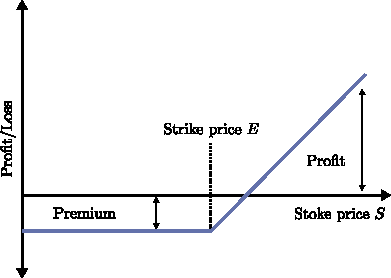
\includegraphics[width=0.45\textwidth]{pay-off.pdf}
  \caption{\label{fig:profit-diagram} Profit diagram for a call option. Adapted from \cite{Wilmott2007}.}
\end{figure}

The profit diagram for a call option is shown in Fig. \ref{fig:profit-diagram}, where the \textbf{premium} is the price paid for contract initially. Then, the 
intrinsic value of the option at the expiration date is calculated as the difference between the stock price $S$ and the strike price $E$. 
This function of the underlying asset is called the \textbf{payoff function} and is given by:
\begin{equation}
  \label{eq:8}
  \text{Payoff} = \max(S - E, 0)
\end{equation}

The purpose of option pricing is to estimate Eq. \ref{eq:8} at the expiration date and then, determine the \textbf{fair value}, which indicates the amount of money an 
investor should pay to enter the option contract today, given the current market conditions. 
The challenging part is to compute the expected value of the option payoff, which is usually done using Monte Carlo methods. In section \ref{sec:literature2} we will discuss the quantum approach to 
this problem.

\subsection{Variational Quantum Algorithms}
Variational Quantum Algorithms (VQAs) are hybrid quantum-classical algorithms that 
are well suited for NISQ devices and allow us to get approximate solutions to optimisation and combinatorial problems efficiently \cite{Cerezo2021}. This algorithms rely on the fact that we can, in 
principle, reformulate any optimisation problem as a QUBO problem \cite{Glover2019}.  

QUBO problems can not directly be cast into a quantum computer, but they share a isomorphism with the Ising Hamiltonian, making it easy to map a QUBO problem into an Ising Hamiltonian, which can be cast into adequate quantum operators in a quantum computer \cite{Buonaiuto2023}. 
\begin{figure}[h!]
\centering 
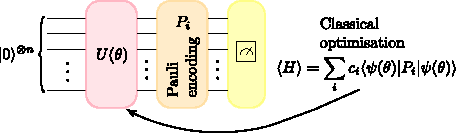
\includegraphics[width=0.5\textwidth]{VQE-Buonaiuto.pdf}
  \caption{\label{fig:vqe} Variational Quantum Eigensolver (VQE) algorithm. Adapted from \cite{Buonaiuto2023}.}
\end{figure}

One of the VQAs used for portfolio optimisation is the Variational Quantum Eigensolver (VQE) algorithm (see Fig. \ref{fig:vqe}). The aim of the VQE algorithm is to find an approximate value for the ground state energy of a given Hamiltonian.  

The starting point is to define a cost function
\begin{equation}
  \label{eq:9}
  C(\boldsymbol{\theta}) =\langle\psi(\boldsymbol{\theta})|H|\psi(\boldsymbol{\theta})\rangle
\end{equation}
where $H$ is the Hamiltonian of our problem, that can be written as the weighted sum of Pauli operators \cite{Tilly2022}, such
\begin{figure*}[ht!]
  \begin{center} 
  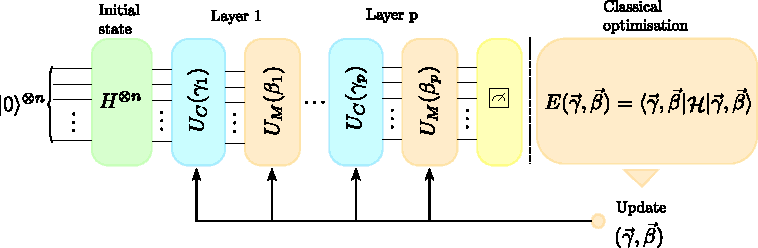
\includegraphics[width=0.85\textwidth]{QAOA-Blekos.pdf}
  \caption{\label{fig:qaoa} Quantum Approximate Optimisation Algorithm (QAOA). Adapted from \cite{Blekos2024}.}
  \end{center}
\end{figure*}
that: 
\begin{equation}
  \label{eq:10}
  \mathcal{H} = \sum_{i} c_i P_i
\end{equation}
where $P_i \in \{I, X, Y, Z\}^{\otimes N}$ are called Pauli strings and $N$ is the number of qubits, and $c_i$ are the coefficients of the Pauli strings.  Additionally, $\boldsymbol{\theta}$ is a set of trainable parameters for some trial state $|\psi(\boldsymbol{\theta})\rangle = U(\boldsymbol{\theta}) |0\rangle ^{\otimes n}$. So, Eq. \ref{eq:9} becomes:
\begin{equation}
  \label{eq:11}
  C(\boldsymbol{\theta}) =\sum_i c_i \langle \boldsymbol{0}|U(\boldsymbol{\theta})^\dagger P_i U(\boldsymbol{\theta})|\boldsymbol{0}\rangle
\end{equation}
for some ansatz $U(\boldsymbol{\theta})$, that can be written as
\begin{equation}
  \label{eq:12}
  U(\boldsymbol{\theta}) = \prod_{k=1}^{p} e^{-i\theta_k \mathcal{H}_k}
\end{equation}
where $\mathcal{H}_k$ are the terms of the Hamiltonian $\mathcal{H}$  and $p$ determines the precision of the approximation \cite{Cerezo2021}.

Therefore, the VQE consists of classical algorithm that uses a quantum algorithm as a subroutine. We first initialise the state 
$|\psi(\boldsymbol{\theta})\rangle$ with some initial parameters $\boldsymbol{\theta}$, then we measure Eq. \ref{eq:11} and use a classical optimisation algorithm to update 
the parameters $\boldsymbol{\theta}$ until we reach a minimum value of $C(\boldsymbol{\theta})$.

The variational principle ensures that at some point the VQE algorithm will converge to:
\begin{equation}
  \label{eq:13}
  E_0 \leq \frac{\langle \psi(\boldsymbol{\theta})|\mathcal{H}|\psi(\boldsymbol{\theta})\rangle}{\langle \psi(\boldsymbol{\theta})|\psi(\boldsymbol{\theta})\rangle}
\end{equation}
where $E_0$ is the ground state energy of the Hamiltonian $\mathcal{H}$ and $|\psi(\boldsymbol{\theta})\rangle$ is some trial state.

In a similar fashion, the Quantum Approximate Optimisation Algorithm (QAOA) is another VQA that was first 
proposed by Farhi et al. \cite{Farhi2014} for combinatorial optimisation problems (e.g. Max-Cut).

Mathematically, we can see the combinatorial optimisation problem as a graph with $m$ edges and $n$ vertices (see Fig. \ref{fig:combinatorial}). Then, define a binary string $x = \{x_1,\cdots, x_n\}$ with $x_i \in \{0, 1\}$. 
\begin{figure}[h!]
\centering 
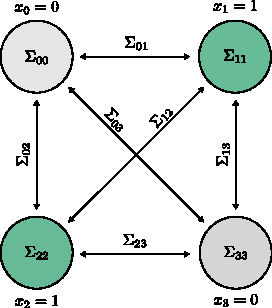
\includegraphics[width=0.35\textwidth]{combinatorial-problem.pdf}
  \caption{\label{fig:combinatorial} A graph representation of a combinatorial optimisation problem with $n =4$ vertices and $m=6$ edges. Adapted from \cite{Baker2022}.} 
\end{figure}
The goal is to find the binary string that maximises the objective function: 
\begin{equation}
  \label{eq:14}
  C(x) = \sum_{i,j=1}^{n} \Sigma_{i,j} x_i (1-x_j)
\end{equation}

In Fig. \ref{fig:qaoa} we show the general structure of the QAOA. First, it initialise $n$ states as a uniform superposition
\begin{equation}
  \label{eq:15}
  |+\rangle^{\otimes n} = \frac{1}{\sqrt{2^n}} \sum_{x} |x\rangle 
\end{equation}
and then, it applies a sequence of $p$ anzates $U(\boldsymbol{\gamma}, \boldsymbol{\beta})$  that are defined as 
\begin{equation}
  \label{eq:16}
  U(\boldsymbol{\gamma}, \boldsymbol{\beta}) = \prod_{k=1}^{p} e^{-i\beta_k \mathcal{H}_M} e^{-i\gamma_k \mathcal{H}_C}
\end{equation}
where $\mathcal{H}_M$ and $\mathcal{H}_C$ are the mixing and cost Hamiltonians, respectively. $\mathcal{H}_C$ encodes the cost function of the problem and $\mathcal{H}_M$ helps guide the optimisation in Hilbert space towards ground state of $\mathcal{H}_C$ \cite{Moll2018}. Similar to the VQE, $\mathcal{H}_C$ can de defined by Eq. \ref{eq:10} and the mixer Hamiltonian 
is defined as $\mathcal{H}_M = -\sum_{i} \sigma_i^x$ \cite{Moll2018}.

After applying the anzates $p$ times, we measure the expectation value of the cost Hamiltonian $C(\boldsymbol{\gamma},\boldsymbol{\beta}) = \langle \psi(\boldsymbol{\gamma}, \boldsymbol{\beta})|\mathcal{H}_C|\psi(\boldsymbol{\gamma},\boldsymbol{\beta})\rangle$ and use a classical optimisation algorithm to update the parameters $\boldsymbol{\gamma}$ and $\boldsymbol{\beta}$ until we reach a minimum value of $C(\boldsymbol{\gamma},\boldsymbol{\beta})$.

\subsection{Quantum Amplitude Estimation}

Quantum Amplitude Estimation (QAE) is an algorithm that can estimate a parameter $a$ with a convergence rate of $\mathcal{O}(1/M)$, where $M$ is the number of samples, which corresponds to a quadratic speedup compared to classical methods (i.e Monte Carlo) which requires $\mathcal{O}(1/\sqrt{M})$ \cite{Egger2020}.  QAE is based on a unitary operator $\mathcal{A}$  that acts on $(n+1)$ qubits such that 
\begin{equation}
  \label{eq:17}
  \mathcal{A}|0\rangle_{n+1} = \sqrt{1-a}|\psi_0\rangle_n|0\rangle + \sqrt{a}|\psi_1\rangle_n|1\rangle
\end{equation}
for some normalised states $|\psi_0\rangle_n$ and $|\psi_1\rangle_n$, where $a \in [0,1]$ is unknown \cite{Stamatopoulos2020}. We can then, 
infer the value of $a$ by performing multiple measurements on $|\Psi\rangle$ and obtaining the ratio of the good state. This method does not represent any advantage with respect to the classical method since the number of queries is exactly the same.  

Therefore, QAE is used along with the amplitude amplification algorithm to amplify the probability of measuring the good state. We achieve that by applying the following operator: 
\begin{equation}
  \label{eq:18}
  \mathcal{Q} = -\mathcal{A} \mathcal{S}_0 \mathcal{A} \mathcal{S}_{\chi}
\end{equation}
where $\mathcal{S}_0$ is the inversion about the mean operator and $\mathcal{S}_{\chi}$ is the oracle operator that flips the sign of the good state \cite{Suzuki2020}.

By defining $\theta_a \in [0, 2\pi]$  so that $a = \sin^2(\theta_a)$, and applying repeatedly $\mathcal{Q}$ for $m$ times on $|\Psi\rangle$  results in
\begin{equation}
  \label{eq:19}
\begin{aligned}
  \mathcal{Q}^m |\Psi\rangle  &= \sin((2m + 1)\theta_a)|\psi_1\rangle_n|1\rangle\\
  & + \cos((2m + 1)\theta_a)|\psi_0\rangle_n|0\rangle 
\end{aligned}
\end{equation}
once measured we can apply a maximum likelihood estimation to infer the value of $a$ \cite{Suzuki2020}.

\section{Classical Approaches}\label{sec:literature1}

In this section we review the main classical approaches to portfolio optimisation and option pricing. 
This section is not intended to be an detailed review on the topic, but rather to provide a point of comparison with the quantum approaches in Sec. \ref{sec:literature2}

\subsection{Portfolio Optimisation}

Classical approaches for portfolio optimisation are based on the MVPO (discussed in Sec. \ref{sec:background}).  
Shadabfar and  Cheng \cite{Shadabfar2020} proposed a probabilistic method for portfolio optimisation using a hybrid Monte Carlo simulation and Markowitz model. They use the cost function defined by Eq. 
\ref{eq:6}, and apply a Monte Carlo to generate multiple random samples of the asset allocations. Then, using the Markowitz optimisation model they computed the optimum values of return and risk for each portfolio. 
\begin{figure}[h!]
\centering 
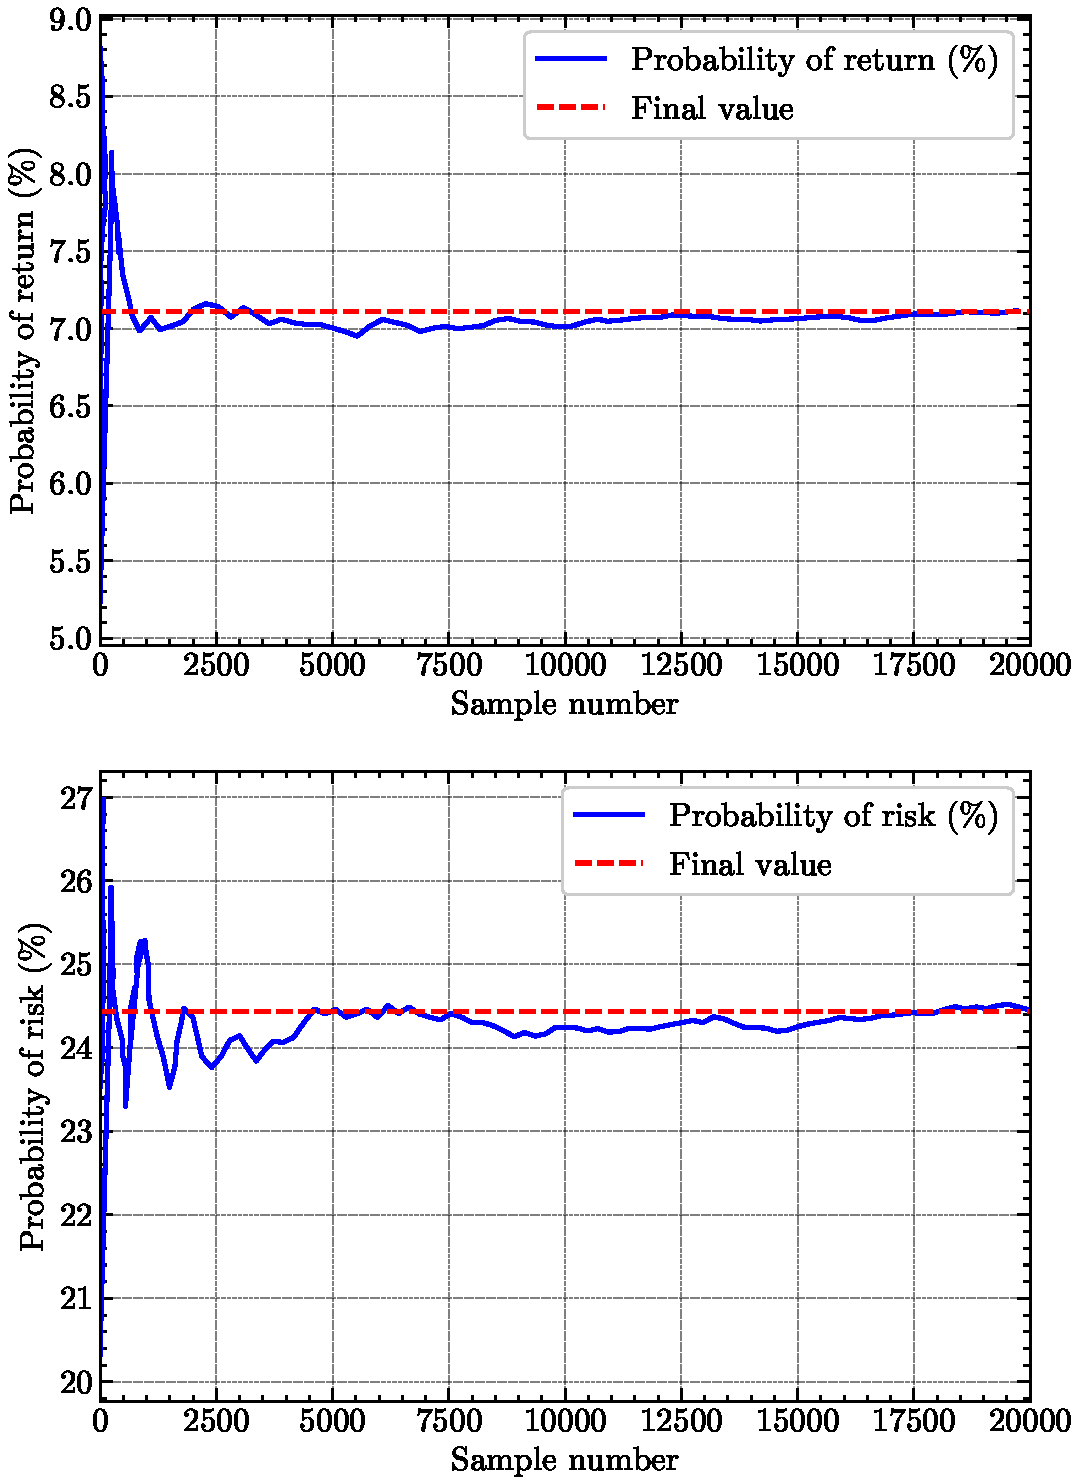
\includegraphics[width=0.5\textwidth]{return-risk-error.pdf}
  \caption{\label{fig:monte-carlo} Convergence of the probabilistic method proposed by Shadabfar and Cheng. The convergence of the return and risk probability depends on the number of random samples considered. Adapted from \cite{Shadabfar2020}.} 
\end{figure}

As shown in Fig. \ref{fig:monte-carlo}, they found that the convergence of their method is dependent on the number of samples used in the Monte Carlo method. Additionally, they demonstrated that the model results 
are roubust to errors in the model's input data, indicating the stability and reliability of their method.

\subsection{Option Pricing}

 The most common classical approach to option pricing are the Monte Carlo methods. In contrast to the Black-Scholes model, which can provide 
 analytical solutions for very simplistic cases, Monte Carlo methods due to their random nature can model and capture the 
 complex behaviour of the financial markets. 

Stochastic differential equations (SDEs) are used to model the evolution of the underlying asset price. The most common SDE used for this task is the Geometric Brownian Motion (GBM) model \cite{Sood2019}, which is given by:
\begin{equation}
  \label{eq:20}
  S_{t+1} = S_t \exp\left(\left[\mu - \frac{1}{2}\sigma^2\right]\Delta t + \sigma \sqrt{\Delta t}Z_t\right)
\end{equation}
where $S_t$ is the asset price at time $t$, $\mu$ is the expected return, $\sigma$ is the volatility, $\Delta t$ is the time step, and $Z_t$ is a standard normal random variable.

The general idea of this method is to simulate the asset price evolution multiple times and calculate the payoff of the option at the expiration date (See Fig. \ref{fig:monte-carlo-option}). The expected value of the option price is then calculated as the average of the payoffs.
\begin{figure}[h!]
\centering
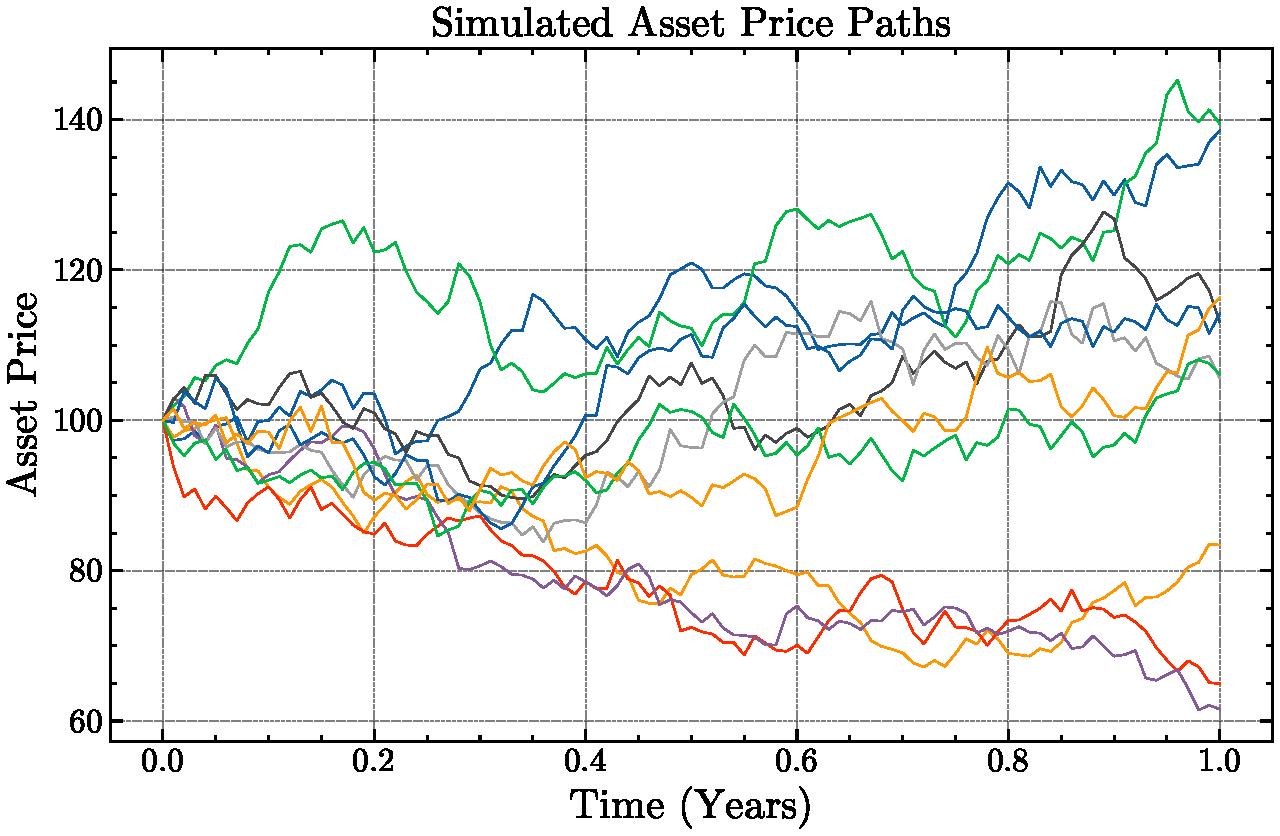
\includegraphics[width=0.5\textwidth]{monte-carlo-paths.pdf}
  \caption{\label{fig:monte-carlo-option} Monte Carlo simulation of the option price for a maturity time $T =1$ (years). The option price is calculated as the average of the payoffs of the option at the expiration date. Adapted from \cite{Sood2019}.}
\end{figure}

In general, the estimation error goes as $\mathcal{O}(1/\sqrt{M})$, where $M$ is the number of samples used in the Monte Carlo simulation. Therefore, we need to find a balance between the estimation error and the time required to compute all the random samples. Although a simplified version of the Monte Carlo method is provided in this section, 
this is the basis for more complex methods. 

\section{Quantum Approaches}\label{sec:literature2}
Having reviewed the classical approaches for both portfolio optimisation and option pricing, it is time to 
introduce the quantum approaches to these problems. In this section we will review the implementations of the quantum algorithms discussed in Sec. \ref{sec:background} for these tasks.
\subsection{Portfolio Optimisation}
In 2023, Buonaiuto et al. \cite{Buonaiuto2023} published a paper where they implemented the VQE algorithm in multiple simulations and in real quantum computers. They used four assets (Apple, IBM, Netflix and Tesla) 
historical data, and the MVPO model to state the optimisation problem. 
\begin{figure}[h!]
\centering 
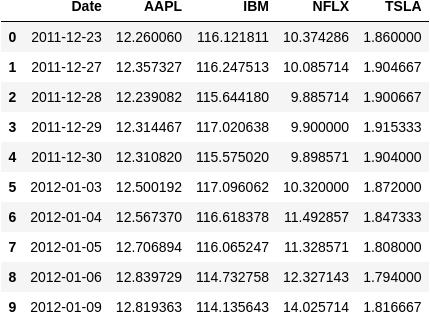
\includegraphics[width=0.45\textwidth]{data-paper.png}
  \caption{\label{fig:data-set} Sample of the historical data of of the assets Apple, IBM, Netflix and Tesla used for the VQE implementation by 
Biunaiuto et al. \cite{Buonaiuto2023}.}
\end{figure}

They mapped the MVPO problem into a QUBO problem (Eq. \ref{eq:21} and Eq. \ref{eq:22}), and then converted it into quantum operators using 
the Ising Hamiltonian, as proposed by \cite{Tilly2022}.  Prices, returns, and covariance matrix of the assets were calculated using the historical data (see Fig. \ref{fig:data-set}). 
\begin{equation}
  \label{eq:21}
  \max_{b} \mathcal{L}(b) =\max_{b}\left(\mu''^{T} b - qb^{T} \Sigma'' b - \lambda(P''^{T}b- 1)^2\right)
\end{equation}
\begin{equation}
  \label{eq:22}
  \mathcal{H} = \sum_{i} h_i Z_i + \sum_{i,j} J_{ij} Z_i\otimes Z_j + \lambda \left(\sum_{i}\pi_i Z_i -\beta\right)^2
\end{equation}

The total expendable budget was set to $B=2000$ for all the experiments, a risk aversion parameter $q=0.5$ was considered. The initial ansatz parameters were randomly selected between $[-\pi, \pi]$. A number of 200 epochs was set, and a penalty parameter $\lambda=10$  was chosen. Finally, the Coybla classical optimiser was used. 

The results of the VQE implementation are shown in Fig. \ref{fig:results}. The results were contrasted with a classical solution. The Toronto, Kolkata and Auckland quantum computers performances perfectly match the classical result. Different ansatz were used for the different quantum computers. 
\begin{figure*}[t!]
\centering
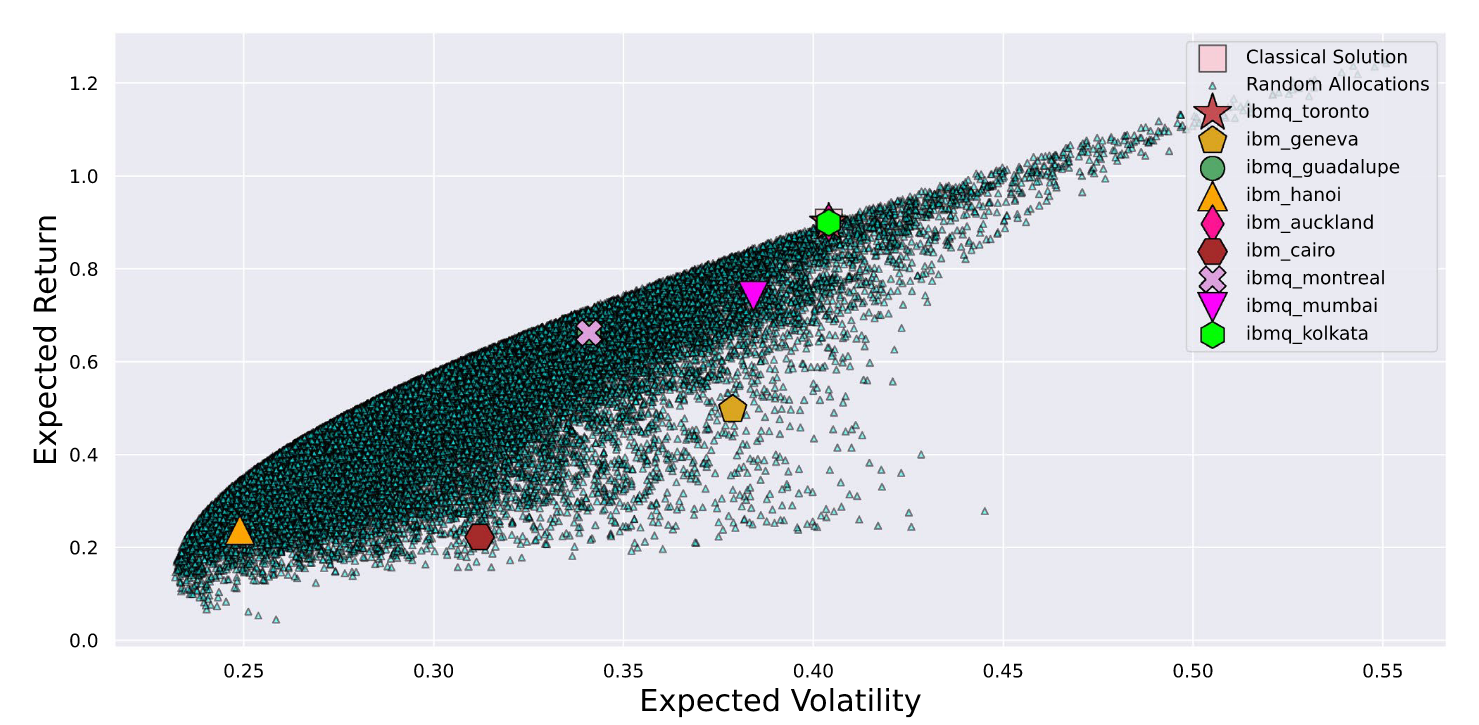
\includegraphics[width=.90\textwidth]{results-vqe.png}
  \caption{\label{fig:results} Results of the VQE implementation by Buonaiuto et al. \cite{Buonaiuto2023}. The optimal asset allocation for the four assets considered is shown. Extracted from 
  \cite{Buonaiuto2023}}
\end{figure*}

\subsection{Option Pricing}
In 2020, Stamatopoulos et al. \cite{Stamatopoulos2020} published a work where they presented a methodology to price options and portfolios of options on a gate-based quantum computer using the QAE algorithm. They implemented their methodology using the IBM Q Tokyo quantum device. Among 
the options covered in their work, they considered multi-asset options and path dependent options.

They discussed the QAE implementation along with the quantum Fourier transform. In their work, they prove mathematically the potential speedup the QAE algorithm could provide compared to the classical Monte Carlo methods, which is in agreement with \cite{Woerner2019, Nakaji2020,Rebentrost2018, Rebentrost2022}. All these works suggest that the estimation error of QAE goes as $\mathcal{O}(1/M)$, whereas the classical Monte Carlo method provides an estimation error that scales as $\mathcal{O}(1/\sqrt{M})$, where $M$ is the number of samples.

Instead of using the QFT, the approach proposed by Suzuki et al. \cite{Suzuki2020} and discussed in Sec. \ref{sec:background} was considered.
Results of the QAE implementation are shown in Fig. \ref{fig:results-qae}. The authors point out the good performance of this algorithm compared to the classical MC.

Furthermore, they used their methodology to price a portfolio of options. They used these results to experimentally prove the speedup of the QAE algorithm (see Fig. \ref{fig:portfolio-option}).

\begin{figure}[h!]
\centering
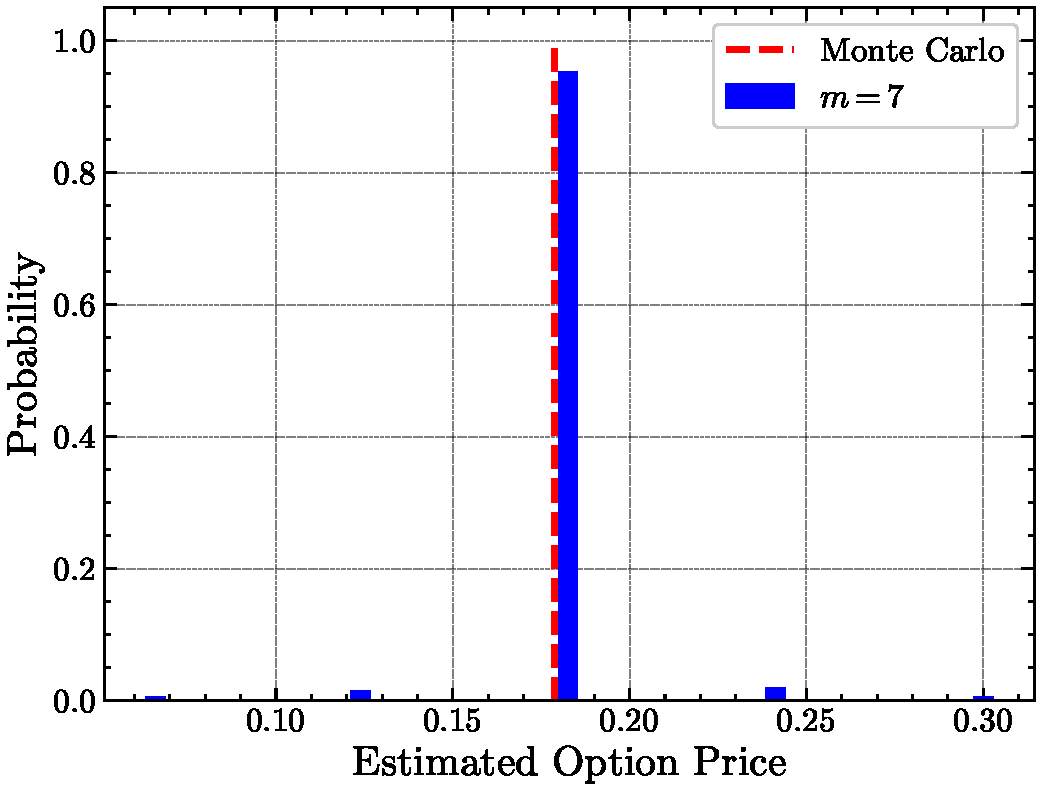
\includegraphics[width=0.45\textwidth]{option-price-estimation.pdf}
  \caption{\label{fig:results-qae} Estimated option price using QAE. $S_0 = 2$, $ \sigma = 10\%$, $r = 4\%$ and $T=300/365$ were used. The red dotted line is the value computed using classical Monte Carlo, and the blue bars represent the estimated option price using QAE after 100000 samples. Adapted  from \cite{Stamatopoulos2020}.}
\end{figure}

\begin{figure}[h!]
\centering
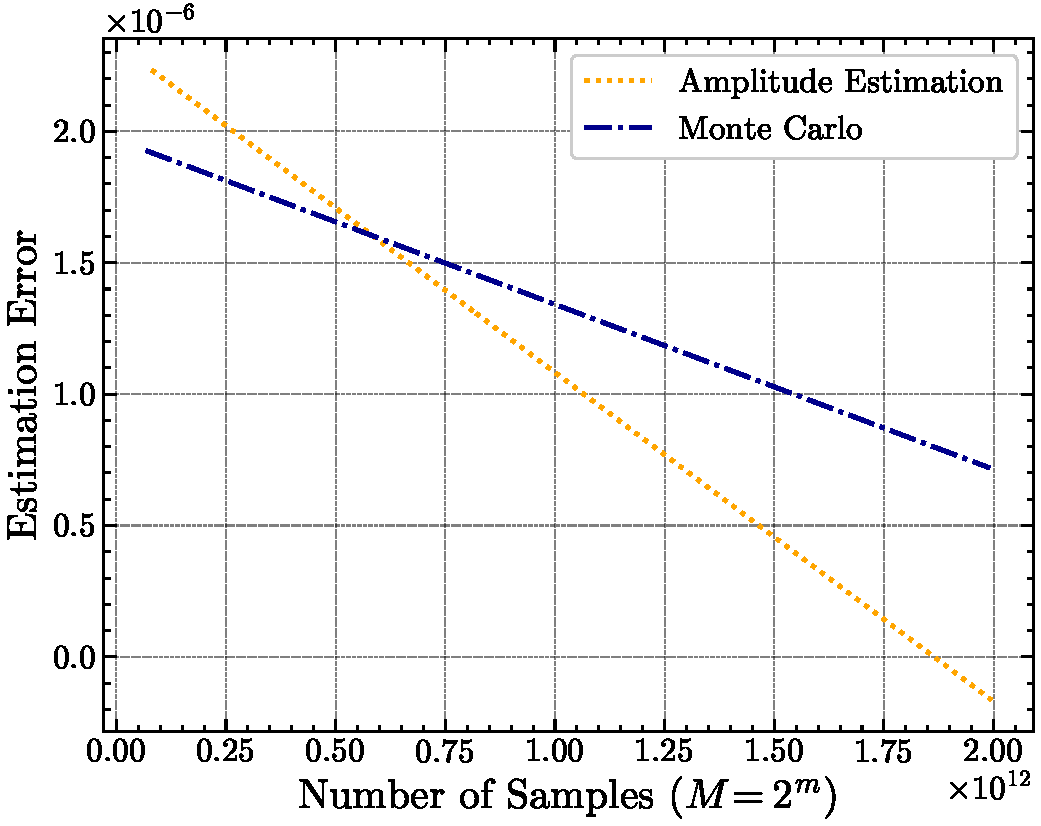
\includegraphics[width=0.45\textwidth]{estimation-error.pdf}
  \caption{\label{fig:portfolio-option} 
Convergence of the estimation error of the option price for a portfolio of options is shown. The yellow dotted line shows the error convergence for the QAE, whereas the blue dashed line indicates the error convergence for the classical Monte Carlo. Adapted  from \cite{Stamatopoulos2020}.}
\end{figure}

\section{Discussion and Conclusion}\label{sec:discussion}
In this work we have reviewed the quantum algorithms proposed for financial applications. Algorithms such as the VQAs and QAE have demonstrated a potential application for portfolio optimisation and option pricing problems. 

VQAs have been successfully implemented for optimisation problems. The results show that the performance of these algorithms is highly dependent on the ansatz structure and hardware topology. Nevertheless, the performance of the VQAs is formidable even when no error mitigation protocol is considered, making them a good candidate for exploiting the computational power that NISQi devices offer to date.  

On the other hand, QAE has been experimentally proven to provide a quadratic speedup over the classical Monte Carlo methods. Applied to 
option pricing, this algorithm has the potential to provide a significant benefit in terms of time and computational 
resources.

Finally, although the results of the quantum algorithms applied to financial applications are promising, 
hardware limitations must be addressed as well as the development of error mitigation protocols. These  implementation results 
show the potential of quantum algorithms beyond the theoretical framework, and pave the way for future research and 
applications in the financial industry.

\FloatBarrier

\bibliography{/home/pacman/Documents/git-repositories/quantum-computing/lecture-notes/bibliography.bib}

\end{document} 
